\documentclass[11pt,letterpaper]{article}
\usepackage[lmargin=1in,rmargin=1in,tmargin=1in,bmargin=1in]{geometry}
\usepackage{../style/homework}
\usepackage{../style/commands}
\setbool{quotetype}{true} % True: Side; False: Under
\setbool{hideans}{true} % Student: True; Instructor: False

% -------------------
% Content
% -------------------
\begin{document}

\homework{6: Due 03/09}{Always remember that you are absolutely unique---just like everyone else.}{Margaret Mead}

% Problem 1
\problem{10} Given the feasible region shown below, find the minimum value of $f(x_1, x_2)= 8x_1 + 6x_2$. Does the function $f(x_1, x_2)$ have a maximum value on the same feasible set? Explain. 
	\[
	\fbox{
	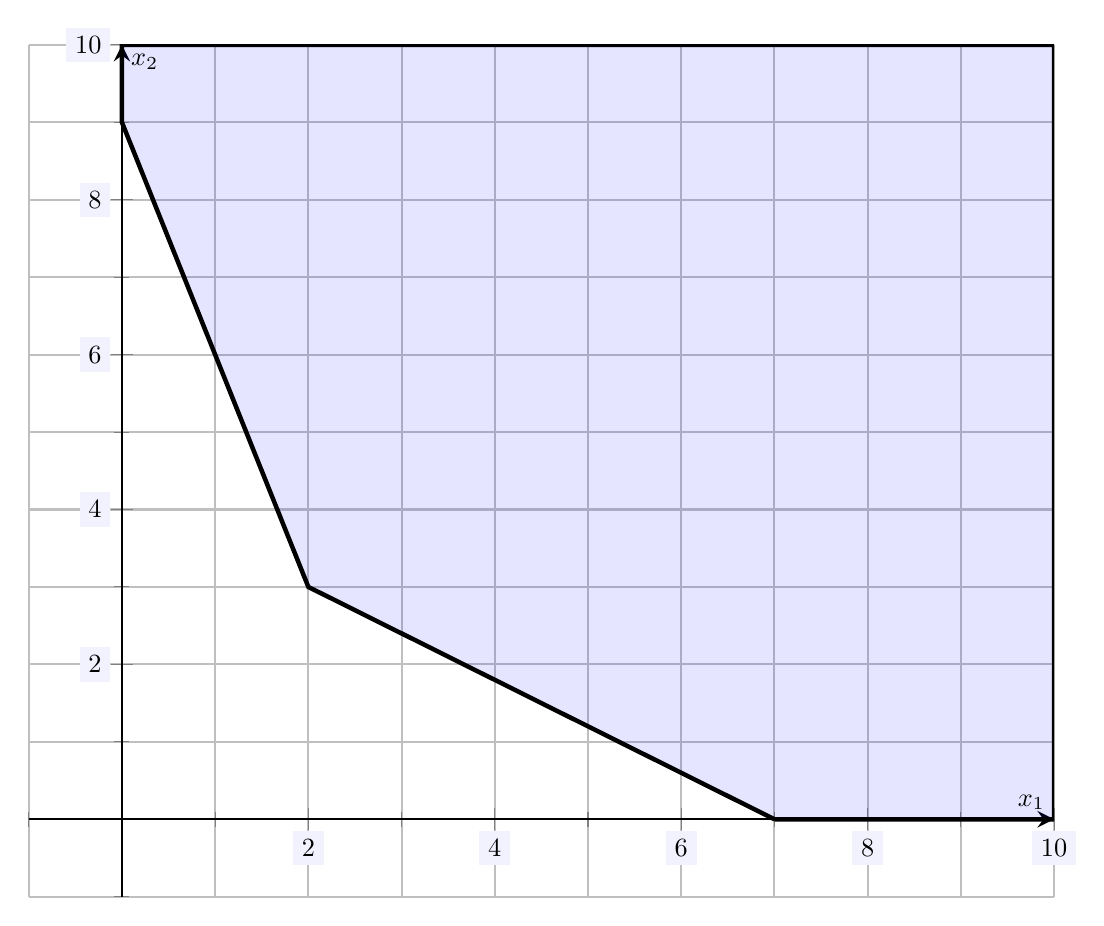
\begin{tikzpicture}[scale=1.9,every node/.style={scale=0.5}]
	\begin{axis}[
	grid=both,
	axis lines=middle,
	ticklabel style={fill=blue!5!white},
	xmin= -1, xmax=10,
	ymin= -1, ymax=10,
	xtick={0,2,4,6,8,10},
	ytick={0,2,4,6,8,10},
	minor tick = {-1,0,1,...,10},
	xlabel=\(x_1\),ylabel=\(x_2\),
	]
	\draw[line width=0.01cm,fill= blue,opacity=0.1] (7,0) -- (2,3) -- (0,9) -- (0,10) -- (10,10) -- (10,0) -- (7,0);
	\draw[line width=0.03cm] (7,0) -- (2,3) -- (0,9) -- (0,10) -- (10,10) -- (10,0) -- (7,0);
	\end{axis}
	\end{tikzpicture}
	}
	\]



\newpage


% Problem 2
\problem{10} Consider the minimization problem given below. As accurately as possible, sketch the feasible region given by the minimization problem. Is this minimization problem in standard form? Explain. Is there a guaranteed solution to this minimization problem? Explain. 
	\[
	\begin{aligned}
	\text{min } z= -3x_1 &+ 8x_2 \\
	x_1 - x_2&\geq -5 \\
	7x_1 + x_2&\leq 35 \\
	x_1, x_2&\geq 0
	\end{aligned}
	\]
	\[
	\fbox{
	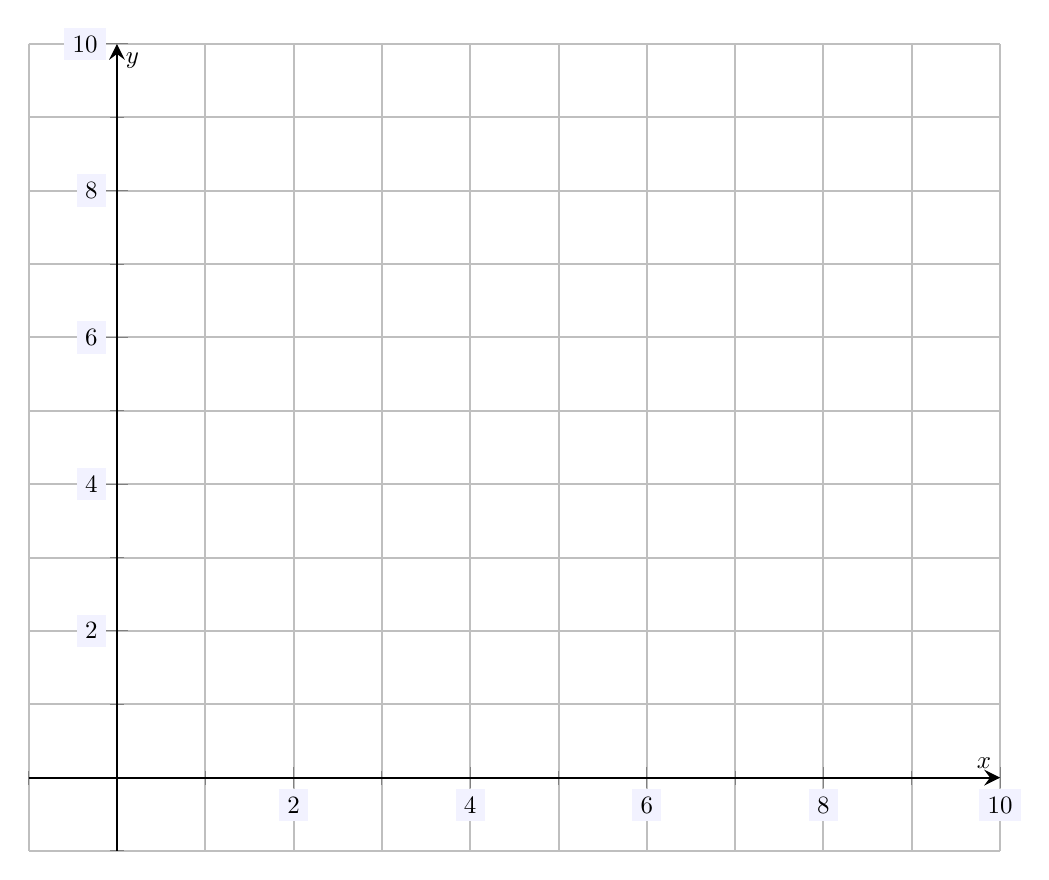
\begin{tikzpicture}[scale=1.8,every node/.style={scale=0.5}]
	\begin{axis}[
	grid=both,
	axis lines=middle,
	ticklabel style={fill=blue!5!white},
	xmin= -1, xmax=10,
	ymin= -1, ymax=10,
	xtick={0,2,4,6,8,10},
	ytick={0,2,4,6,8,10},
	minor tick = {-1,0,1,...,10},
	xlabel=\(x\),ylabel=\(y\),
	]
	\end{axis}
	\end{tikzpicture}
	}
	\]





\newpage



% Problem 3
\problem{10} Assume the following is an `initial simplex tableau associated to a standard minimization problem.' Write down the function being maximized and the corresponding system of constraints. Explain how the function and corresponding system of constraints changes if the problem were a standard maximization problem.
	\begin{table}[!ht]
	\centering
	\begin{tabular}{rrrrrr|r}
	$4$ & $-2$ & $6$ & $5$ & $1$ & $0$ & $125$ \\
	$3$ & $0$ & $-3$ & $5$ & $0$ & $1$ & $340$ \\ \hline
	$-1$ & $3$ & $-2$ & $-6$ & $0$ & $0$ & $0$ 
	\end{tabular}
	\end{table}



\newpage



% Problem 4
\problem{10} Find the dual problem to\dots
	\[
	\begin{aligned}
	\text{min } w= 6x_1 - 7x_2 &+ 9x_3 \\
	x_1 + 7x_2 - x_3&\geq 10 \\
	2x_1 - 4x_3&\geq 5 \\
	x_1 + 5x_2 + 4x_3&\geq 10 \\
	x_1, x_2, x_3&\geq 0 
	\end{aligned}
	\]


\end{document}